\Problem{Representations of Volume}{\VolReps}{
You want to determine the volume of the room you are in.
}
\ProblemSub{\VolRepsA}{
(a) Write a description of how to find the volume of the room in words.
}
\Solution{\VolRepsASol}{

If we measure the dimensions of the room (ceiling height, length, width), and multiply them together, we can get a decent estimate of the volume of the room.

Of course, it won't be perfect. The floor isn't even, the walls have a few pillars embedded in them, the doors lie in slight recesses, and there are air ducts sticking into the room. We could find their volumes and subtract, perhaps, if we need that level of accuracy.

Instead, we will assume for simplicity that the room is rectangular and empty.
}
\ProblemSub{\VolRepsB}{
(b) Sketch a diagram that would help you find the volume of the room.
}
\Solution{\VolRepsBSol}{

\begin{figure}[h]
	\centering
	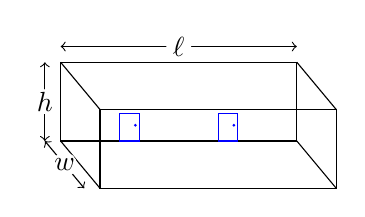
\begin{tikzpicture}
		\begin{scope}
			\coordinate (nearll) at (0,0);
			\coordinate (nearlr) at (3,0);
			\coordinate (nearur) at (3,1);
			\coordinate (nearul) at (0,1);
			\draw (nearll) -- (nearlr) -- (nearur) -- (nearul) -- cycle;
		\end{scope}
		\begin{scope}[shift={(-0.5,0.6)}]
			\coordinate (farll) at (0,0);
			\coordinate (farlr) at (3,0);
			\coordinate (farur) at (3,1);
			\coordinate (farul) at (0,1);
			\draw (farll) -- (farlr) -- (farur) -- (farul) -- cycle;
			\draw[<->] (0,1.2) -- (3,1.2);
			\filldraw[white] (1.5,1.2) circle (0.15);
			\node at (1.5,1.2) {$\ell$};
			\draw[<->] (-0.2,0) -- (-0.2,1);
			\filldraw[white] (-0.2,0.5) circle (0.15);
			\node at (-0.2,0.5) {$h$};
			\begin{scope}[shift={(0.75,0)}]
				\draw[blue] (0,0) -- (0.25,0) -- (0.25,0.35) -- (0,0.35) -- cycle;
				\draw[blue] (0.2,0.2) circle (0.01);
			\end{scope}
			\begin{scope}[shift={(2,0)}]
				\draw[blue] (0,0) -- (0.25,0) -- (0.25,0.35) -- (0,0.35) -- cycle;
				\draw[blue] (0.2,0.2) circle (0.01);
			\end{scope}
		\end{scope}
		\draw (nearll) -- (farll);
		\draw (nearlr) -- (farlr);
		\draw (nearur) -- (farur);
		\draw (nearul) -- (farul);
		\draw[<->] (-0.2,0) -- (-0.7,0.6);
		\filldraw[white] (-0.45,0.3) circle (0.15);
		\node at (-0.45,0.3) {$w$};
	\end{tikzpicture}
\end{figure}

I put the {\color{blue}doors} in to orient the drawing. They are otherwise not critical, and their sizes and positions are not quantitatively accurate.
}
\ProblemSub{\VolRepsC}{
(c) Write a symbolic expression that would allow you to find the volume of the room. Check the units of your expression.
}
\Solution{\VolRepsCSol}{

\[
V = \ell w h
\]
Length $\ell$, width $w$, and height $h$ are all lengths, which would be measured in meters in SI units. Volume is measured in m$^{3}$ in SI units. When we multiply $\ell w h$, we are multiplying meters by meters by meters, which gives us m$^{3}$, so we have the same units on either side of the equal sign:
\[
[V] = \text{m}^{3}, \qquad [\ell w h] = [\ell][w][h]=\text{m}\cdot\text{m}\cdot\text{m}=\text{m}^{3}.
\]
}
\ProblemSub{\VolRepsD}{
(d) Without standing up, estimate the volume of the room as a number. Make sense of the number by comparing it to something.
}
\Solution{\VolRepsDSol}{

There are several ways to estimate the dimensions of the room without measuring it directly:
\begin{itemize}
	\item Guess your local TA's height (or just ask) and compare them to the height of the ceiling, like a living measuring stick.
	\item Look up the height of a standard interior door (Home Depot says 80 inches, which is about 2.032 meters) and estimate how many doors high the ceiling is.
	\item The carpet tiles are a regular size. Measure one nearby and count how many you see from one wall to another.
\end{itemize}
For comparison, an Olympic pool is about 2500 m$^{3}$ (technically, there is no standard depth, so this can vary). Comparing this to the size of the room can give you some idea about how accurate your estimate is (for example, the room is certainly not larger than an Olympic pool).
}